\documentclass[11pt,a4paper]{article}

\usepackage[utf8]{inputenc}
\usepackage[T1]{fontenc}
\usepackage[spanish]{babel}
\usepackage{amsmath}
\usepackage{amsfonts}
\usepackage{amssymb}
\usepackage{graphicx}
\usepackage{tabularx}
\usepackage{booktabs}
\usepackage{hyperref}
\usepackage{geometry}
\usepackage{listings}
\usepackage{xcolor}
\usepackage{caption}
\usepackage{subcaption}
\usepackage{titlesec}
\usepackage{parskip}
\usepackage{float}

% Configuración de títulos de párrafos
\titleformat{\paragraph}[hang]
{\normalfont\normalsize\bfseries}{\theparagraph}{1em}{}
\titlespacing*{\paragraph}
{0pt}{3.25ex plus 1ex minus .2ex}{1em}

\geometry{top=3cm, bottom=3cm, left=2.5cm, right=2.5cm}

\hypersetup{
    colorlinks=true,
    linkcolor=black,
    filecolor=magenta,      
    urlcolor=cyan,
}

\definecolor{codegreen}{rgb}{0,0.6,0}
\definecolor{codegray}{rgb}{0.5,0.5,0.5}
\definecolor{codepurple}{rgb}{0.58,0,0.82}
\definecolor{backcolour}{rgb}{0.95,0.95,0.92}

\lstdefinestyle{mystyle}{
    backgroundcolor=\color{backcolour},   
    commentstyle=\color{codegreen},
    keywordstyle=\color{magenta},
    numberstyle=\tiny\color{codegray},
    stringstyle=\color{codepurple},
    basicstyle=\ttfamily\small,
    breakatwhitespace=false,         
    breaklines=true,                 
    captionpos=b,                    
    keepspaces=true,                 
    numbers=left,                    
    numbersep=5pt,                  
    showspaces=false,                
    showstringspaces=false,
    showtabs=false,                  
    tabsize=2
}

\lstset{style=mystyle}

\begin{document}
\begin{titlepage}
    \begin{center}
        \vspace*{1cm}

        \Huge
        \textbf{Laboratorio N°2}

        \vspace{0.5cm}
        \LARGE
        Filtro FIR con FRDM-MCXN947

        \vspace{1.5cm}

        \vfill

        \Large
        \textbf{Autor:} Simón Saillen

        \Large
        \textbf{Profesores:} Gustavo Parlanti, Roberto Rossi, German Molina, Pablo Ferreira

        \vspace{0.5cm}

        \Large
        \textbf{Procesamiento Digital de Señales}\\
        \vspace{0.2cm}
        \textbf{FCEFyN -- UNC}\\
        \vspace{0.2cm}
        2026

    \end{center}
\end{titlepage}
\newpage

\section{Introducción}

\section{Consigna}

Realizar un programa aplicativo que sea capaz de aplicar un filtro FIR por
muestras a un buffer de memoria de 512 muestras, que es adquirido con el
\textit{Laboratorio 1} teniendo en cuenta las frecuencias de muestro de
\texttt{8 kS/s}, \texttt{16 kS/s}, \texttt{22 kS/s}, \texttt{44 kS/s} y
\texttt{48 kS/s}.

Con una de las teclas de la placa se habilitara la aplicacion del filtro FIR o
se hace bypass del filtro a un buffer de salida distinto del buffer de entrada.
De este buffer de salida se enviaran las muestras al DAC.\@

Visualizar el resultado utilizando un osciloscopio y comparar los resultados.

\textbf{Requerimientos de los Filtros:}

\begin{itemize}
    \item Pasa Bajos: $f_c = 3600 [\text{Hz}]$, $A_{stop} = 30 [\text{dB}]$
    \item Pasa Altos: $f_c = 35 [\text{Hz}]$, $A_{stop} = 30 [\text{dB}]$
    \item Pasa Banda: $f_{c1} = 35 [\text{Hz}]$, $f_{c2} = 3500 [\text{Hz}]$, $A_{stop} =
              30 [\text{dB}]$
    \item Elimina Banda: $f_r = 50 [\text{Hz}]$, $BW = 15 [\text{Hz}]$, $A_{stop} = 25
                  [\text{dB}]$
\end{itemize}

\section{Desarrollo}

La configuracion inicial de los pines, clocks y perifericos necesarios resulta
igual a la del \textit{Laboratorio 1}, siendo esta:

\subsection{Configuración de Clocks}

Principalmente se deben configurar los clocks de la placa, ya que todos los
modulos de la misma dependen de esta configuracion. Para ello se utilizara
dentro de ConfigTools el modulo \texttt{CLOCK} del SDK de NXP, el cual permite
configurar los distintos clocks de la placa.

\begin{table}[H]
    \centering
    \begin{tabular}{|c|c|c|c|}
        \hline
        \textbf{Clock Component} & \textbf{Frequency} & \textbf{Clock Source} & \textbf{Description}        \\
        \hline
        MAIN\_clock              & 150 MHz            & PLL0                  & Clock principal de la placa \\
        ADC0\_clock              & 48 MHz             & Fast IRC              & Clock del modulo ADC        \\
        DAC0\_clock              & 48 MHz             & Fast IRC              & Clock del modulo DAC        \\
        CTIMER0\_clock           & 150 MHz            & PLL0                  & Clock del modulo Timer      \\
        FLEXXCOM4\_clock         & 12 MHz             & Slow IRC              & Clock del modulo UART       \\
        \hline
    \end{tabular}
    \caption{Configuración de clocks usando ConfigTools}
\end{table}

El modulo UART se configuro para enviar mensajes de debugging a la PC, por lo
que se utilizo una pre configuracion con un baudrate de \texttt{115200 bps} y
un clock de 12 MHz.

\subsection{Modulo Low-Power ADC (LPADC0)}

El modulo ADC de la placa FRDM-MCXN947 es un conversor de 12 bits de baja
potencia con un rango de voltaje de refencia de 0 a 3.3V. El mismo se configuro
con los siguientes parametros:

\begin{table}[H]
    \centering
    \begin{tabular}{|c|c|c|}
        \hline
        \textbf{Campo}          & \textbf{Valor} & \textbf{Descripcion}                                \\
        \hline
        Pre-enable ADC          & Enabled        & Enciende el circuito analogico con anterioridad     \\
        Autocalibration         & Enabled        & Calibra al iniciar para compensar desviaciones      \\
        Doze mode               & Enabled        & Permite que funcione en modo de bajo consumo        \\
        FIFO 0 watermark        & 1              & Genera interrupcion cuando hay 1 muestra en la FIFO \\
        Enable interrupt vector & Enabled        & Habilita la interrupcion del ADC                    \\
        Interrupt sources       & FIFO 0         & La fuente de interrupcion es la FIFO 0 watermark    \\
        Interrupt priority      & 0              & Prioridad de la interrupcion del ADC                \\
        \hline
    \end{tabular}
    \caption{Configuración General del ADC en ConfigTools/Peripherals}
\end{table}

\begin{table}[H]
    \centering
    \begin{tabular}{|c|c|c|}
        \hline
        \textbf{Campo}      & \textbf{Valor}                  & \textbf{Descripcion}        \\
        \hline
        Command ID          & start\_conversion               & Identificador del comando   \\
        Command number      & 1                               & Numero de comando           \\
        Channel sample mode & Single end mode, using A        & Modo de muestreo            \\
        Channel number      & ADC0\_A0                        & Pin de entrada del ADC      \\
        Resolution mode     & High resolution (16 bits)       & Resolucion de la conversion \\
        Loop count          & 0                               & Ejecuta el comando una vez  \\
        Sample time mode    & 3 ADCK cycles total sample time & Tiempo de muestreo          \\
        \hline
    \end{tabular}
    \caption{Conversion Command del ADC en ConfigTools/Peripherals}
\end{table}

\begin{table}[H]
    \centering
    \begin{tabular}{|c|c|c|}
        \hline
        \textbf{Campo}         & \textbf{Valor}  & \textbf{Descripcion}                  \\
        \hline
        Trigger ID             & timer0\_trigger & Identificador del trigger             \\
        Trigger number         & 0               & Numero de trigger                     \\
        Trigger command number & 1               & Numero de comando a ejecutar          \\
        High priority          & Enabled         & Ejecuta el comando con prioridad alta \\
        Select channel A FIFO  & FIFO 0          & Habilita la FIFO A del ADC            \\
        Delay value            & 0               & No hay delay entre trigger y comando  \\
        \hline
    \end{tabular}
    \caption{Trigger Command del ADC en ConfigTools/Peripherals}
\end{table}

\subsection{Modulo Timer (CTIMER0)}

El modulo CTIMER0 es un timer de 32 bits que se utiliza para generar el trigger
de conversión del ADC.\@ Se configuró desde Peripherals en ConfigTools con los
siguientes parámetros:

\begin{table}[H]
    \centering
    \begin{tabular}{|c|c|c|}
        \hline
        \textbf{Campo}          & \textbf{Valor}           & \textbf{Descripcion}               \\
        \hline
        Timer mode              & Timer (bus clock source) & Modo de funcionamiento             \\
        Prescaler value         & 1                        & Frecuencia de clock del timer      \\
        Match channel           & 0                        & Canal de match del timer           \\
        Match value             & 18750 ($\approx 8kHz$)   & Valor de match del timer           \\
        Reset on match          & Enabled                  & Resetea el timer al hacer match    \\
        Match interrupt request & Enabled                  & Genera interrupcion al hacer match \\
        Interrupt priority      & 1                        & Prioridad de la interrupcion       \\
        \hline
    \end{tabular}
    \caption{Configuración del Timer en ConfigTools/Peripherals}
\end{table}

El match value inicial corresponde a la velocidad de muestreo de \texttt{8
    kS/s}, posteriorment con el uso de los switch este valor es cambiado para
cumplir con las velocidades de muestreo requeridas.

\subsubsection{Segundo Modulo Timer (CTIMER1)}

Tambien se configuro un segundo timer (CTIMER1) para generar la señal de
parpadeo del LED RGB, el mismo se configura con un match value dependiendo del
filtro seleccionado, para que el parpadeo del LED indique el filtro activo.

Su configuracion es similar a la del CTIMER0, con la diferencia de que el match
value se actualiza segun el filtro seleccionado, y la prioridad de la
interrupcion es menor que la del CTIMER0, para no interrumpir ni la aplicacion
de filtro ni la adquisicion de muestras del ADC.\@

\subsection{Modulo Low-Power DAC (LPDAC0)}

El modulo DAC de la placa es un conversor digital a analógico de 12 bits con un
rango de voltaje de salida de 0 a 3.3V. El mismo se configuró desde Peripherals
en ConfigTools con los siguientes parámetros:

\begin{table}[H]
    \centering
    \begin{tabular}{|c|c|c|}
        \hline
        \textbf{Campo}             & \textbf{Valor} & \textbf{Descripcion}                     \\
        \hline
        Enable DAC                 & Enabled        & Habilita el modulo DAC                   \\
        Reference voltage source   & VREF\_INT      & Fuente de voltaje de referencia          \\
        Opamp as buffer            & Enabled        & Habilita el buffer de salida             \\
        Enable LPDAC               & Enabled        & Habilita el modo de bajo consumo         \\
        Set LPDAC level after init & Enabled        & Configura el nivel de salida al encender \\
        LPDAC level                & 0              & Nivel de salida inicial del DAC (0V)     \\
        \hline
    \end{tabular}
    \caption{Configuración del DAC en ConfigTools/Peripherals}
\end{table}

\subsection{Filtros FIR (Finite Impulse Response)}

La Respuesta en el Tiempo de un Filtro FIR se calcula a partir de la
ponderación de las muestras presentes y pasadas con los coeficientes del
filtro. Los coeficientes son la caracterizacion del filtro, variando estos se
pueden obtener los distintos tipos de filtros (pasa bajos, pasa altos, etc.).

La ecuacion caracteristica de un filtro FIR es la siguiente:

\begin{equation}
    y[n] = \sum_{k=0}^{N-1} h[k] \cdot x[n-k]
\end{equation}

Teniendo:

\begin{itemize}
    \item $y[n]$: Salida del filtro en el instante de tiempo $n$.
    \item $x[n-k]$: Entrada del filtro en el instante de tiempo $n-k$.
    \item $h[k]$: Coeficiente del filtro en el instante de tiempo $k$.
    \item $N$: Cantidad de taps (logitud del filtro).
\end{itemize}

\subsection{Metodo de Ventana: Kaiser}

El metodo de la ventana es el metodo mas comun para el diseño de filtros FIR
debido a su simplicidad y facilidad de implementacion. Una ventana consiste en
un arreglo de valores finitos que conforman los coeficientes que satisfacen los
requerimientos de diseño del filtro.

La \textit{Ventana de Kaiser} es una aproximacion a la ventana esferoidal
prolata, para la que se maximiza la relacion de energia del lobulo principal y
se minimiza la relación de energia del lobulo lateral.

Para lograr una atenuacion relativa del lobulo lateral de $A_{stop}$, el
parametro $\beta$ de la ventana de Kaiser se calcula con la siguiente ecuacion:

\begin{equation}
    \beta = \begin{cases}
        0.1102(A_{stop} - 8.7),                                 & A_{stop} > 50            \\
        0.5842{(A_{stop} - 21)}^{0.4} + 0.07886(A_{stop} - 21), & 50 \geq A_{stop} \geq 21 \\
        0,                                                      & A_{stop} < 21
    \end{cases}
\end{equation}

Y podemos calcular el orden (o longitud) del filtro con la siguiente ecuacion:

\begin{equation}
    N = \frac{A_{stop} - 8}{2.285 \cdot 2\pi(BW/f_s)} + 1
\end{equation}

El calculo de los coeficientes del filtro se realizo usando GNU/Octave,
utilizando la funcion \texttt{fir1} con la ventana de Kaiser, el script
utilizado se encuentra en \texttt{fir\_coefficients.m}.

En la siguiente tabla se muestran los parametros de diseño de cada filtro
FIR:\@

\begin{table}[H]
    \centering
    \begin{tabular}{|c|c|c|}
        \hline
        \textbf{Filtro}    & \textbf{Beta} & \textbf{Orden (N)} \\
        \hline
        Pasa Bajos (LP)    & 2.1166        & 76                 \\
        Pasa Altos (HP)    & 2.1166        & 151                \\
        Pasa Banda (BP)    & 2.1166        & 150                \\
        Rechaza Banda (BS) & 0             & 571                \\
        \hline
    \end{tabular}
\end{table}

Estos coeficientes son los que se cargan en la memoria de la placa para ser
utilizados por el filtro FIR.\@

Los coeficientes son convertidos a formato Q15 para ser utilizados en la placa,
esto se hace multiplicando los valores por $2^{15}$ y redondeando al entero mas
cercano, luego se limita el valor a el rango de -32768 a 32767.

Los filtros diseñados se muestran en las siguientes figura, donde se puede
observar la respuesta en frecuencia de cada uno de ellos en Magnitud y Fase.

Los filtros pasabanda y rechazabanda tienen similitud con los filtros pasabajos
y pasaaltos debido a que la frecuencia de corte de estos filtros es muy baja en
comparacion con la frecuencia de muestreo, haciendo muy poco visible la banda
de paso y la banda de rechazo.

\begin{figure}[H]
    \centering
    \hfill
    \begin{subfigure}[b]{0.49\textwidth}
        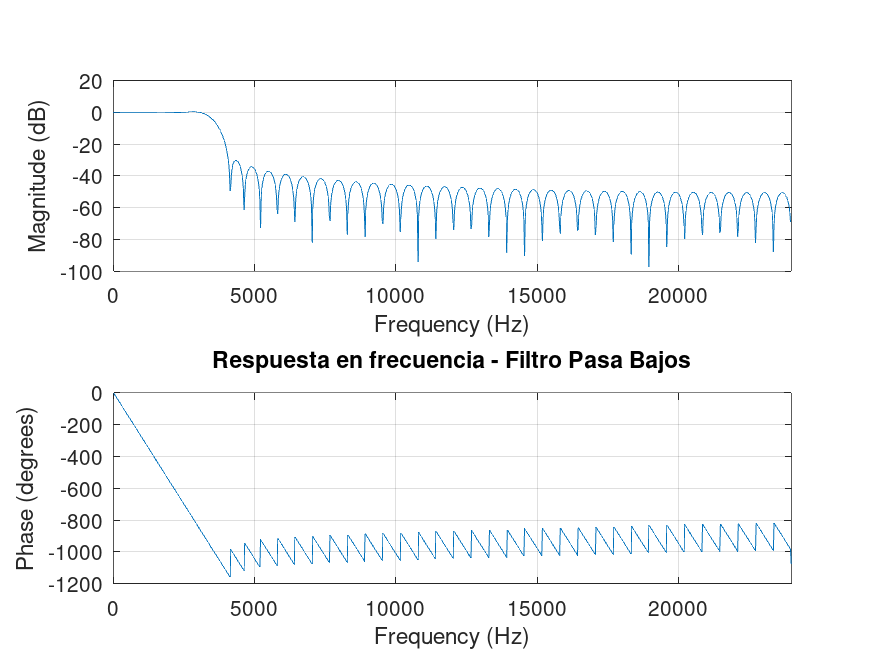
\includegraphics[width=\textwidth]{../images/FIR_LP.png}
    \end{subfigure}
    \hfill
    \begin{subfigure}[b]{0.49\textwidth}
        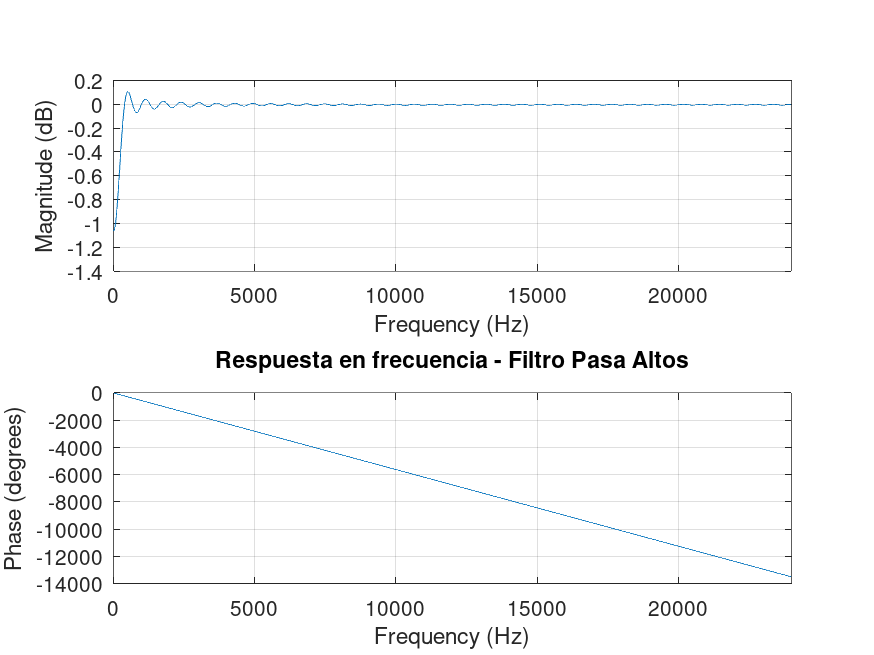
\includegraphics[width=\textwidth]{../images/FIR_HP.png}
    \end{subfigure}
    \hfill
    \caption{Filtros Pasabajo (Izquierda) y Pasaaltos (Derecha)}
\end{figure}

\begin{figure}[H]
    \centering
    \hfill
    \begin{subfigure}[b]{0.49\textwidth}
        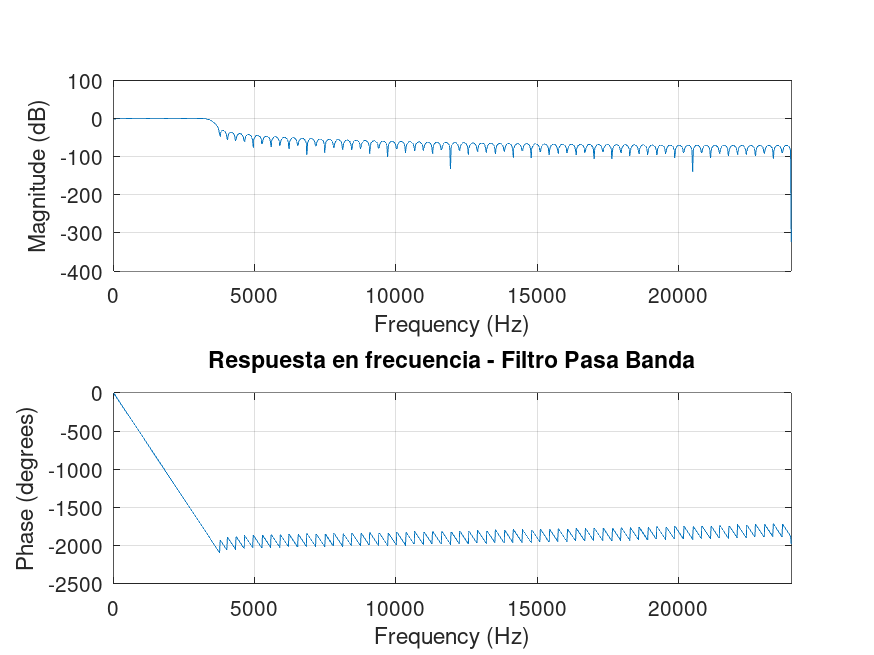
\includegraphics[width=\textwidth]{../images/FIR_BP.png}
    \end{subfigure}
    \hfill
    \begin{subfigure}[b]{0.49\textwidth}
        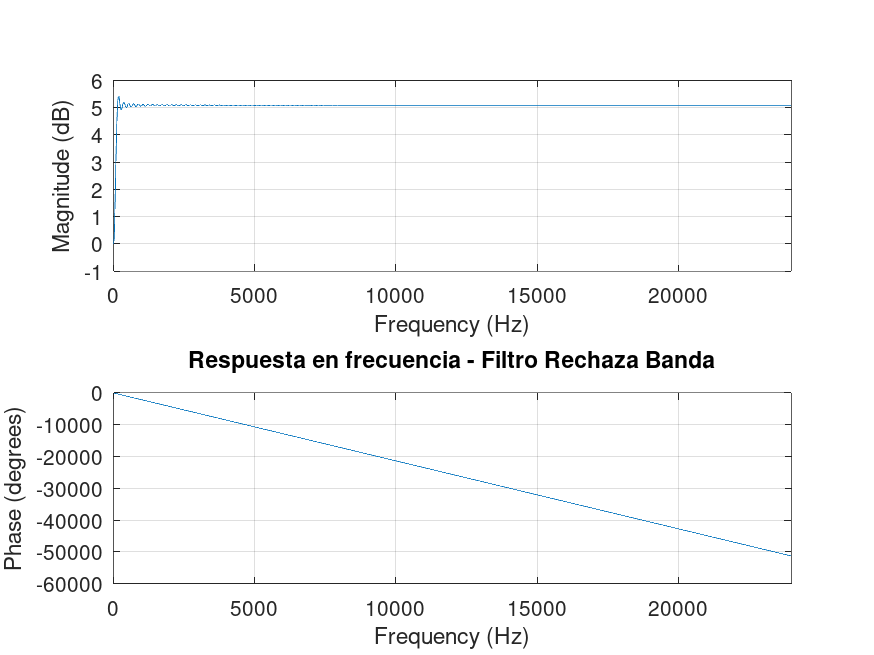
\includegraphics[width=\textwidth]{../images/FIR_BS.png}
    \end{subfigure}
    \hfill
    \caption{Filtros Pasa Banda (Izquierda) y Rechaza Banda (Derecha)}
\end{figure}

\subsection{Programa Principal}

El programa principal implementa un sistema de filtrado FIR en tiempo real
utilizando interrupciones y buffers circulares. La arquitectura se basa en tres
componentes principales:

\subsubsection{Buffers de memoria}

Se utilizan dos buffers circulares de 512 muestras en formato Q15:

\begin{itemize}
    \item \texttt{input\_buffer}: Almacena las muestras crudas capturadas por el ADC.
    \item \texttt{output\_buffer}: Almacena las muestras filtradas que se envian al DAC.
\end{itemize}

\subsubsection{Flujo de datos}

El flujo de datos en el sistema es el siguiente:

\begin{enumerate}
    \item El Timer0 genera un trigger periodico segun la frecuencia de muestreo
          seleccionada.
    \item La interrupcion del Timer0 lee la siguiente muestra de \texttt{input\_buffer},
          aplica el filtro FIR seleccionado (o bypass si esta deshabilitado), guarda el
          resultado en \texttt{output\_buffer} y lo envia al DAC.
    \item Al finalizar, Timer0 dispara al ADC para la siguiente conversion.
    \item La interrupcion del ADC almacena la muestra cruda en \texttt{input\_buffer}.
\end{enumerate}

El ADC siempre escribe sobre el buffer de entrada en una posicion arriba de
donde lee el Timer0, de esta manera se asegura que el Timer0 siempre lea un
dato valido.

\subsubsection{Filtros FIR con CMSIS DSP}

Los filtros se implementan utilizando la libreria CMSIS DSP, especificamente
las funciones \texttt{arm\_fir\_init\_q15} y \texttt{arm\_fir\_q15}.

El filtrado se realiza muestra por muestra (\texttt{blockSize = 1}), lo que
simplifica la implementacion en el contexto de interrupciones pero incrementa
la sobrecarga por llamada a funcion.

\subsubsection{Control por teclado}

\begin{itemize}
    \item \textbf{SW3 (GPIO00\_IRQHandler)}: Cicla entre los filtros en orden
          \texttt{OFF $\rightarrow$ LP $\rightarrow$ HP $\rightarrow$ BP $\rightarrow$
              BS $\rightarrow$ OFF}. Al cambiar de filtro, se actualiza el valor de
          match del Timer1 para modificar la velocidad de parpadeo del LED.
    \item \textbf{SW2 (GPIO01\_IRQHandler)}: Cicla entre las frecuencias de
          muestreo: \texttt{8 $\rightarrow$ 16 $\rightarrow$ 22 $\rightarrow$ 44
              $\rightarrow$ 48 kS/s}. Actualiza el valor de match del Timer0 para
          cambiar el periodo de muestreo.
\end{itemize}

\subsubsection{Indicacion visual}

Para visualizar la configuracion del sistema, tanto en filtro aplicado como en
velocidad de muestreo, se utiliza el LED RGB en conjunto con configuraciones de
parpadeo.

Las siguientes tablas muestran la correspondencia entre color y velocidad de
muestreo, y entre parpadeo y filtro aplicado.

\begin{table}[H]
    \centering
    \begin{tabular}{|c|c|c|}
        \hline
        \textbf{Velocidad de muestreo} & \textbf{Color del LED} & \textbf{Configuracion RGB} \\
        \hline
        8 kS/s                         & \color{green}VERDE     & R = 100                    \\
        16 kS/s                        & \color{blue}AZUL       & B = 100                    \\
        22 kS/s                        & \color{yellow}AMARILLO & R = 100, G = 100           \\
        44 kS/s                        & \color{red}ROJO        & G = 100                    \\
        48 kS/s                        & \color{magenta}MAGENTA & R = 100, B = 100           \\
        \hline
    \end{tabular}
    \caption{Colores del LED RGB integrados de la placa}
\end{table}

\begin{table}[H]
    \centering
    \begin{tabular}{|c|c|c|}
        \hline
        \textbf{Filtro Aplicado} & \textbf{Parpadeo} \\
        \hline
        OFF                       & Sin parpadeo      \\
        LP                        & 1 segundo         \\
        HP                        & 0.75 segundos     \\
        BP                        & 0.5 segundos      \\
        BS                        & 0.25 segundos     \\
        \hline
    \end{tabular}
    \caption{Parpadeo del LED RGB integrados de la placa segun el filtro aplicado}
\end{table}

\section{Resultados}

\subsection{Capturas de osciloscopio}

% TODO: Agregar capturas del osciloscopio mostrando:
% - Señal de entrada (sin filtro)
% - Señal filtrada con cada uno de los 4 filtros
% - Comparar a distintas frecuencias de muestreo

\subsection{Graficas de Octave}

% TODO: Agregar capturas de las respuestas en frecuencia generadas por Octave

\section{Conclusiones}

% TODO: Completar con conclusiones del laboratorio

\begin{thebibliography}{9}
    \bibitem{kaiser_window}
    MathWorks (MATLAB). Kaiser Window.\\
    \url{https://la.mathworks.com/help/signal/ug/kaiser-window.html}

    \bibitem{mikroe_window}
    MikroElektronika. Window Functions.\\
    \url{https://www.mikroe.com/ebooks/digital-filter-design/window-functions}
\end{thebibliography}

\end{document}